\documentclass[1p]{elsarticle_modified}
%\bibliographystyle{elsarticle-num}

%\usepackage[colorlinks]{hyperref}
%\usepackage{abbrmath_seonhwa} %\Abb, \Ascr, \Acal ,\Abf, \Afrak
\usepackage{amsfonts}
\usepackage{amssymb}
\usepackage{amsmath}
\usepackage{amsthm}
\usepackage{scalefnt}
\usepackage{amsbsy}
\usepackage{kotex}
\usepackage{caption}
\usepackage{subfig}
\usepackage{color}
\usepackage{graphicx}
\usepackage{xcolor} %% white, black, red, green, blue, cyan, magenta, yellow
\usepackage{float}
\usepackage{setspace}
\usepackage{hyperref}

\usepackage{tikz}
\usetikzlibrary{arrows}

\usepackage{multirow}
\usepackage{array} % fixed length table
\usepackage{hhline}

%%%%%%%%%%%%%%%%%%%%%
\makeatletter
\renewcommand*\env@matrix[1][\arraystretch]{%
	\edef\arraystretch{#1}%
	\hskip -\arraycolsep
	\let\@ifnextchar\new@ifnextchar
	\array{*\c@MaxMatrixCols c}}
\makeatother %https://tex.stackexchange.com/questions/14071/how-can-i-increase-the-line-spacing-in-a-matrix
%%%%%%%%%%%%%%%

\usepackage[normalem]{ulem}

\newcommand{\msout}[1]{\ifmmode\text{\sout{\ensuremath{#1}}}\else\sout{#1}\fi}
%SOURCE: \msout is \stkout macro in https://tex.stackexchange.com/questions/20609/strikeout-in-math-mode

\newcommand{\cancel}[1]{
	\ifmmode
	{\color{red}\msout{#1}}
	\else
	{\color{red}\sout{#1}}
	\fi
}

\newcommand{\add}[1]{
	{\color{blue}\uwave{#1}}
}

\newcommand{\replace}[2]{
	\ifmmode
	{\color{red}\msout{#1}}{\color{blue}\uwave{#2}}
	\else
	{\color{red}\sout{#1}}{\color{blue}\uwave{#2}}
	\fi
}

\newcommand{\Sol}{\mathcal{S}} %segment
\newcommand{\D}{D} %diagram
\newcommand{\A}{\mathcal{A}} %arc


%%%%%%%%%%%%%%%%%%%%%%%%%%%%%5 test

\def\sl{\operatorname{\textup{SL}}(2,\Cbb)}
\def\psl{\operatorname{\textup{PSL}}(2,\Cbb)}
\def\quan{\mkern 1mu \triangleright \mkern 1mu}

\theoremstyle{definition}
\newtheorem{thm}{Theorem}[section]
\newtheorem{prop}[thm]{Proposition}
\newtheorem{lem}[thm]{Lemma}
\newtheorem{ques}[thm]{Question}
\newtheorem{cor}[thm]{Corollary}
\newtheorem{defn}[thm]{Definition}
\newtheorem{exam}[thm]{Example}
\newtheorem{rmk}[thm]{Remark}
\newtheorem{alg}[thm]{Algorithm}

\newcommand{\I}{\sqrt{-1}}
\begin{document}

%\begin{frontmatter}
%
%\title{Boundary parabolic representations of knots up to 8 crossings}
%
%%% Group authors per affiliation:
%\author{Yunhi Cho} 
%\address{Department of Mathematics, University of Seoul, Seoul, Korea}
%\ead{yhcho@uos.ac.kr}
%
%
%\author{Seonhwa Kim} %\fnref{s_kim}}
%\address{Center for Geometry and Physics, Institute for Basic Science, Pohang, 37673, Korea}
%\ead{ryeona17@ibs.re.kr}
%
%\author{Hyuk Kim}
%\address{Department of Mathematical Sciences, Seoul National University, Seoul 08826, Korea}
%\ead{hyukkim@snu.ac.kr}
%
%\author{Seokbeom Yoon}
%\address{Department of Mathematical Sciences, Seoul National University, Seoul, 08826,  Korea}
%\ead{sbyoon15@snu.ac.kr}
%
%\begin{abstract}
%We find all boundary parabolic representation of knots up to 8 crossings.
%
%\end{abstract}
%\begin{keyword}
%    \MSC[2010] 57M25 
%\end{keyword}
%
%\end{frontmatter}

%\linenumbers
%\tableofcontents
%
\newcommand\colored[1]{\textcolor{white}{\rule[-0.35ex]{0.8em}{1.4ex}}\kern-0.8em\color{red} #1}%
%\newcommand\colored[1]{\textcolor{white}{ #1}\kern-2.17ex	\textcolor{white}{ #1}\kern-1.81ex	\textcolor{white}{ #1}\kern-2.15ex\color{red}#1	}

{\Large $\underline{11n_{184}~(K11n_{184})}$}

\setlength{\tabcolsep}{10pt}
\renewcommand{\arraystretch}{1.6}
\vspace{1cm}\begin{tabular}{m{100pt}>{\centering\arraybackslash}m{274pt}}
\multirow{5}{120pt}{
	\centering
	\includegraphics[width=112pt]{../../../GIT/diagram.site/Diagrams/png/800_11n_184.png}\\
\ \ \ A knot diagram\footnotemark}&
\allowdisplaybreaks
\textbf{Linearized knot diagam} \\
\cline{2-2}
 &
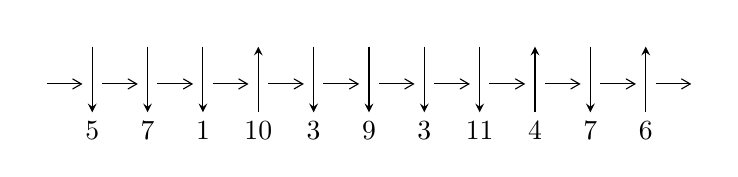
\begin{tikzpicture}[x=20pt, y=17pt]
	% nodes
	\node (C0) at (0, 0) {};
	\node (C1) at (1, 0) {};
	\node (C1U) at (1, +1) {};
	\node (C1D) at (1, -1) {5};

	\node (C2) at (2, 0) {};
	\node (C2U) at (2, +1) {};
	\node (C2D) at (2, -1) {7};

	\node (C3) at (3, 0) {};
	\node (C3U) at (3, +1) {};
	\node (C3D) at (3, -1) {1};

	\node (C4) at (4, 0) {};
	\node (C4U) at (4, +1) {};
	\node (C4D) at (4, -1) {10};

	\node (C5) at (5, 0) {};
	\node (C5U) at (5, +1) {};
	\node (C5D) at (5, -1) {3};

	\node (C6) at (6, 0) {};
	\node (C6U) at (6, +1) {};
	\node (C6D) at (6, -1) {9};

	\node (C7) at (7, 0) {};
	\node (C7U) at (7, +1) {};
	\node (C7D) at (7, -1) {3};

	\node (C8) at (8, 0) {};
	\node (C8U) at (8, +1) {};
	\node (C8D) at (8, -1) {11};

	\node (C9) at (9, 0) {};
	\node (C9U) at (9, +1) {};
	\node (C9D) at (9, -1) {4};

	\node (C10) at (10, 0) {};
	\node (C10U) at (10, +1) {};
	\node (C10D) at (10, -1) {7};

	\node (C11) at (11, 0) {};
	\node (C11U) at (11, +1) {};
	\node (C11D) at (11, -1) {6};
	\node (C12) at (12, 0) {};

	% arrows
	\draw[->,>={angle 60}]
	(C0) edge (C1) (C1) edge (C2) (C2) edge (C3) (C3) edge (C4) (C4) edge (C5) (C5) edge (C6) (C6) edge (C7) (C7) edge (C8) (C8) edge (C9) (C9) edge (C10) (C10) edge (C11) (C11) edge (C12) ;	\draw[->,>=stealth]
	(C1U) edge (C1D) (C2U) edge (C2D) (C3U) edge (C3D) (C4D) edge (C4U) (C5U) edge (C5D) (C6U) edge (C6D) (C7U) edge (C7D) (C8U) edge (C8D) (C9D) edge (C9U) (C10U) edge (C10D) (C11D) edge (C11U) ;
	\end{tikzpicture} \\
\hhline{~~} \\& 
\textbf{Solving Sequence} \\ \cline{2-2} 
 &
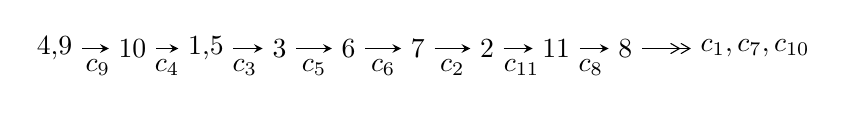
\begin{tikzpicture}[x=25pt, y=7pt]
	% node
	\node (A0) at (-1/8, 0) {4,9};
	\node (A1) at (1, 0) {10};
	\node (A2) at (33/16, 0) {1,5};
	\node (A3) at (25/8, 0) {3};
	\node (A4) at (33/8, 0) {6};
	\node (A5) at (41/8, 0) {7};
	\node (A6) at (49/8, 0) {2};
	\node (A7) at (57/8, 0) {11};
	\node (A8) at (65/8, 0) {8};
	\node (C1) at (1/2, -1) {$c_{9}$};
	\node (C2) at (3/2, -1) {$c_{4}$};
	\node (C3) at (21/8, -1) {$c_{3}$};
	\node (C4) at (29/8, -1) {$c_{5}$};
	\node (C5) at (37/8, -1) {$c_{6}$};
	\node (C6) at (45/8, -1) {$c_{2}$};
	\node (C7) at (53/8, -1) {$c_{11}$};
	\node (C8) at (61/8, -1) {$c_{8}$};
	\node (A9) at (10, 0) {$c_{1},c_{7},c_{10}$};

	% edge
	\draw[->,>=stealth]	
	(A0) edge (A1) (A1) edge (A2) (A2) edge (A3) (A3) edge (A4) (A4) edge (A5) (A5) edge (A6) (A6) edge (A7) (A7) edge (A8) ;
	\draw[->>,>={angle 60}]	
	(A8) edge (A9);
\end{tikzpicture} \\ 

\end{tabular} \\

\footnotetext{
The image of knot diagram is generated by the software ``\textbf{Draw programme}" developed by Andrew Bartholomew(\url{http://www.layer8.co.uk/maths/draw/index.htm\#Running-draw}), where we modified some parts for our purpose(\url{https://github.com/CATsTAILs/LinksPainter}).
}\phantom \\ \newline 
\centering \textbf{Ideals for irreducible components\footnotemark of $X_{\text{par}}$} 
 
\begin{align*}
I^u_{1}&=\langle 
9.79327\times10^{23} u^{27}-1.97941\times10^{24} u^{26}+\cdots+2.45772\times10^{24} b-1.05681\times10^{25},\\
\phantom{I^u_{1}}&\phantom{= \langle  }5.11012\times10^{24} u^{27}-1.51176\times10^{25} u^{26}+\cdots+2.45772\times10^{25} a-1.24464\times10^{26},\;u^{28}-3 u^{27}+\cdots-40 u+10\rangle \\
I^u_{2}&=\langle 
2554960 u^{17} a-4096933 u^{17}+\cdots-42906164 a+49128383,\\
\phantom{I^u_{2}}&\phantom{= \langle  }-103879132 u^{17} a-263156948 u^{17}+\cdots+1344416472 a+157961924,\;u^{18}-8 u^{16}+\cdots-3 u-7\rangle \\
I^u_{3}&=\langle 
-17 u^{17}-10 u^{16}+\cdots+4 b-38,\;u^{17}-11 u^{16}+\cdots+4 a-58,\\
\phantom{I^u_{3}}&\phantom{= \langle  }u^{18}-6 u^{16}+19 u^{14}-40 u^{12}+66 u^{10}-82 u^8+76 u^6-46 u^4+15 u^2-2\rangle \\
I^u_{4}&=\langle 
b+u+1,\;2 a- u-2,\;u^2-2\rangle \\
\\
I^v_{1}&=\langle 
a,\;b-1,\;v+1\rangle \\
\end{align*}
\raggedright * 5 irreducible components of $\dim_{\mathbb{C}}=0$, with total 85 representations.\\
\footnotetext{All coefficients of polynomials are rational numbers. But the coefficients are sometimes approximated in decimal forms when there is not enough margin.}
\newpage
\renewcommand{\arraystretch}{1}
\centering \section*{I. $I^u_{1}= \langle 9.79\times10^{23} u^{27}-1.98\times10^{24} u^{26}+\cdots+2.46\times10^{24} b-1.06\times10^{25},\;5.11\times10^{24} u^{27}-1.51\times10^{25} u^{26}+\cdots+2.46\times10^{25} a-1.24\times10^{26},\;u^{28}-3 u^{27}+\cdots-40 u+10 \rangle$}
\flushleft \textbf{(i) Arc colorings}\\
\begin{tabular}{m{7pt} m{180pt} m{7pt} m{180pt} }
\flushright $a_{4}=$&$\begin{pmatrix}0\\u\end{pmatrix}$ \\
\flushright $a_{9}=$&$\begin{pmatrix}1\\0\end{pmatrix}$ \\
\flushright $a_{10}=$&$\begin{pmatrix}1\\- u^2\end{pmatrix}$ \\
\flushright $a_{1}=$&$\begin{pmatrix}-0.207921 u^{27}+0.615107 u^{26}+\cdots-17.2289 u+5.06419\\-0.398469 u^{27}+0.805384 u^{26}+\cdots-15.8021 u+4.29997\end{pmatrix}$ \\
\flushright $a_{5}=$&$\begin{pmatrix}u\\- u^3+u\end{pmatrix}$ \\
\flushright $a_{3}=$&$\begin{pmatrix}-0.598386 u^{27}+1.36198 u^{26}+\cdots-25.7006 u+6.72775\\-0.0606363 u^{27}+0.102546 u^{26}+\cdots-2.30306 u-0.524423\end{pmatrix}$ \\
\flushright $a_{6}=$&$\begin{pmatrix}0.429997 u^{27}-0.891523 u^{26}+\cdots+10.5673 u-1.39779\\-0.00865581 u^{27}+0.0715894 u^{26}+\cdots-3.25265 u+2.07921\end{pmatrix}$ \\
\flushright $a_{7}=$&$\begin{pmatrix}0.438653 u^{27}-0.963112 u^{26}+\cdots+13.8200 u-3.47700\\-0.00865581 u^{27}+0.0715894 u^{26}+\cdots-3.25265 u+2.07921\end{pmatrix}$ \\
\flushright $a_{2}=$&$\begin{pmatrix}0.0771778 u^{27}+0.0489359 u^{26}+\cdots-7.53802 u+2.27914\\-0.431569 u^{27}+0.843759 u^{26}+\cdots-14.8252 u+4.40618\end{pmatrix}$ \\
\flushright $a_{11}=$&$\begin{pmatrix}0.498943 u^{27}-1.06015 u^{26}+\cdots+13.2218 u-3.30666\\-0.0479065 u^{27}+0.0970119 u^{26}+\cdots-3.79894 u+1.67983\end{pmatrix}$ \\
\flushright $a_{8}=$&$\begin{pmatrix}-0.175255 u^{27}+0.212502 u^{26}+\cdots+2.68490 u-0.0259453\\-0.0725597 u^{27}+0.0693962 u^{26}+\cdots+2.45288 u-0.486297\end{pmatrix}$\\ \flushright $a_{8}=$&$\begin{pmatrix}-0.175255 u^{27}+0.212502 u^{26}+\cdots+2.68490 u-0.0259453\\-0.0725597 u^{27}+0.0693962 u^{26}+\cdots+2.45288 u-0.486297\end{pmatrix}$\\&\end{tabular}
\flushleft \textbf{(ii) Obstruction class $= -1$}\\~\\
\flushleft \textbf{(iii) Cusp Shapes $= -\frac{4877780988340105932664134}{2457723581593567328996461} u^{27}+\frac{9987788121812337009415536}{2457723581593567328996461} u^{26}+\cdots-\frac{189867457763355278132012850}{2457723581593567328996461} u+\frac{43001401194012443714550992}{2457723581593567328996461}$}\\~\\
\newpage\renewcommand{\arraystretch}{1}
\flushleft \textbf{(iv) u-Polynomials at the component}\newline \\
\begin{tabular}{m{50pt}|m{274pt}}
Crossings & \hspace{64pt}u-Polynomials at each crossing \\
\hline $$\begin{aligned}c_{1},c_{10}\end{aligned}$$&$\begin{aligned}
&u^{28}+u^{27}+\cdots+303 u+49
\end{aligned}$\\
\hline $$\begin{aligned}c_{2},c_{7}\end{aligned}$$&$\begin{aligned}
&u^{28}+3 u^{27}+\cdots-120 u+26
\end{aligned}$\\
\hline $$\begin{aligned}c_{3},c_{6}\end{aligned}$$&$\begin{aligned}
&u^{28}- u^{27}+\cdots- u+1
\end{aligned}$\\
\hline $$\begin{aligned}c_{4},c_{9}\end{aligned}$$&$\begin{aligned}
&u^{28}+3 u^{27}+\cdots+40 u+10
\end{aligned}$\\
\hline $$\begin{aligned}c_{5},c_{8}\end{aligned}$$&$\begin{aligned}
&u^{28}- u^{27}+\cdots+21 u+5
\end{aligned}$\\
\hline $$\begin{aligned}c_{11}\end{aligned}$$&$\begin{aligned}
&u^{28}+3 u^{27}+\cdots+56 u+8
\end{aligned}$\\
\hline
\end{tabular}\\~\\
\newpage\renewcommand{\arraystretch}{1}
\flushleft \textbf{(v) Riley Polynomials at the component}\newline \\
\begin{tabular}{m{50pt}|m{274pt}}
Crossings & \hspace{64pt}Riley Polynomials at each crossing \\
\hline $$\begin{aligned}c_{1},c_{10}\end{aligned}$$&$\begin{aligned}
&y^{28}+29 y^{27}+\cdots-8019 y+2401
\end{aligned}$\\
\hline $$\begin{aligned}c_{2},c_{7}\end{aligned}$$&$\begin{aligned}
&y^{28}+23 y^{27}+\cdots-1816 y+676
\end{aligned}$\\
\hline $$\begin{aligned}c_{3},c_{6}\end{aligned}$$&$\begin{aligned}
&y^{28}+y^{27}+\cdots+17 y+1
\end{aligned}$\\
\hline $$\begin{aligned}c_{4},c_{9}\end{aligned}$$&$\begin{aligned}
&y^{28}-17 y^{27}+\cdots+560 y+100
\end{aligned}$\\
\hline $$\begin{aligned}c_{5},c_{8}\end{aligned}$$&$\begin{aligned}
&y^{28}+19 y^{27}+\cdots+379 y+25
\end{aligned}$\\
\hline $$\begin{aligned}c_{11}\end{aligned}$$&$\begin{aligned}
&y^{28}- y^{27}+\cdots+640 y+64
\end{aligned}$\\
\hline
\end{tabular}\\~\\
\newpage\flushleft \textbf{(vi) Complex Volumes and Cusp Shapes}
$$\begin{array}{c|c|c}  
\text{Solutions to }I^u_{1}& \I (\text{vol} + \sqrt{-1}CS) & \text{Cusp shape}\\
 \hline 
\begin{aligned}
u &= -0.892804 + 0.444060 I \\
a &= \phantom{-}0.309008 + 0.559978 I \\
b &= -0.873429 + 0.799710 I\end{aligned}
 & \phantom{-}1.26054 - 1.72230 I & -0.40850 + 1.70276 I \\ \hline\begin{aligned}
u &= -0.892804 - 0.444060 I \\
a &= \phantom{-}0.309008 - 0.559978 I \\
b &= -0.873429 - 0.799710 I\end{aligned}
 & \phantom{-}1.26054 + 1.72230 I & -0.40850 - 1.70276 I \\ \hline\begin{aligned}
u &= \phantom{-}0.218854 + 1.012420 I \\
a &= \phantom{-}0.590636 - 0.144749 I \\
b &= \phantom{-}0.764812 - 0.117020 I\end{aligned}
 & -1.38872 - 0.92374 I & -4.94776 + 7.36786 I \\ \hline\begin{aligned}
u &= \phantom{-}0.218854 - 1.012420 I \\
a &= \phantom{-}0.590636 + 0.144749 I \\
b &= \phantom{-}0.764812 + 0.117020 I\end{aligned}
 & -1.38872 + 0.92374 I & -4.94776 - 7.36786 I \\ \hline\begin{aligned}
u &= \phantom{-}0.802643 + 0.305370 I \\
a &= \phantom{-}0.75217 - 1.24109 I \\
b &= -1.08256 - 1.21911 I\end{aligned}
 & -1.15395 + 4.47162 I & -7.14862 - 4.64379 I \\ \hline\begin{aligned}
u &= \phantom{-}0.802643 - 0.305370 I \\
a &= \phantom{-}0.75217 + 1.24109 I \\
b &= -1.08256 + 1.21911 I\end{aligned}
 & -1.15395 - 4.47162 I & -7.14862 + 4.64379 I \\ \hline\begin{aligned}
u &= \phantom{-}0.584905 + 0.590380 I \\
a &= \phantom{-}0.965167 - 0.178536 I \\
b &= \phantom{-}0.259310 - 0.627636 I\end{aligned}
 & -1.36729 - 0.61050 I & -5.48708 + 0.91172 I \\ \hline\begin{aligned}
u &= \phantom{-}0.584905 - 0.590380 I \\
a &= \phantom{-}0.965167 + 0.178536 I \\
b &= \phantom{-}0.259310 + 0.627636 I\end{aligned}
 & -1.36729 + 0.61050 I & -5.48708 - 0.91172 I \\ \hline\begin{aligned}
u &= \phantom{-}1.216130 + 0.158248 I \\
a &= -0.911081 - 0.448221 I \\
b &= \phantom{-}0.709894 - 0.706039 I\end{aligned}
 & \phantom{-}8.36654 + 1.60580 I & -0.541797 - 0.240729 I \\ \hline\begin{aligned}
u &= \phantom{-}1.216130 - 0.158248 I \\
a &= -0.911081 + 0.448221 I \\
b &= \phantom{-}0.709894 + 0.706039 I\end{aligned}
 & \phantom{-}8.36654 - 1.60580 I & -0.541797 + 0.240729 I\\
 \hline 
 \end{array}$$\newpage$$\begin{array}{c|c|c}  
\text{Solutions to }I^u_{1}& \I (\text{vol} + \sqrt{-1}CS) & \text{Cusp shape}\\
 \hline 
\begin{aligned}
u &= \phantom{-}1.099020 + 0.606761 I \\
a &= -0.148240 - 0.260078 I \\
b &= -0.80758 - 1.16185 I\end{aligned}
 & \phantom{-}7.22801 + 2.43402 I & \phantom{-}1.57040 - 0.59342 I \\ \hline\begin{aligned}
u &= \phantom{-}1.099020 - 0.606761 I \\
a &= -0.148240 + 0.260078 I \\
b &= -0.80758 + 1.16185 I\end{aligned}
 & \phantom{-}7.22801 - 2.43402 I & \phantom{-}1.57040 + 0.59342 I \\ \hline\begin{aligned}
u &= \phantom{-}1.243000 + 0.278668 I \\
a &= \phantom{-}0.112693 - 0.881381 I \\
b &= -0.184859 - 0.444395 I\end{aligned}
 & \phantom{-}2.92454 + 5.00287 I & -4.13660 - 6.40651 I \\ \hline\begin{aligned}
u &= \phantom{-}1.243000 - 0.278668 I \\
a &= \phantom{-}0.112693 + 0.881381 I \\
b &= -0.184859 + 0.444395 I\end{aligned}
 & \phantom{-}2.92454 - 5.00287 I & -4.13660 + 6.40651 I \\ \hline\begin{aligned}
u &= -1.193670 + 0.454674 I \\
a &= \phantom{-}0.069212 + 0.789810 I \\
b &= -0.54519 + 1.66827 I\end{aligned}
 & \phantom{-}7.75458 - 5.65256 I & \phantom{-}3.62489 + 8.19789 I \\ \hline\begin{aligned}
u &= -1.193670 - 0.454674 I \\
a &= \phantom{-}0.069212 - 0.789810 I \\
b &= -0.54519 - 1.66827 I\end{aligned}
 & \phantom{-}7.75458 + 5.65256 I & \phantom{-}3.62489 - 8.19789 I \\ \hline\begin{aligned}
u &= -0.097920 + 0.715313 I \\
a &= \phantom{-}1.130000 + 0.601158 I \\
b &= -0.248100 + 0.524577 I\end{aligned}
 & \phantom{-}4.52132 + 1.28199 I & -1.48628 - 3.62447 I \\ \hline\begin{aligned}
u &= -0.097920 - 0.715313 I \\
a &= \phantom{-}1.130000 - 0.601158 I \\
b &= -0.248100 - 0.524577 I\end{aligned}
 & \phantom{-}4.52132 - 1.28199 I & -1.48628 + 3.62447 I \\ \hline\begin{aligned}
u &= -1.299880 + 0.322120 I \\
a &= -0.777664 - 0.901721 I \\
b &= \phantom{-}1.34969 - 1.28546 I\end{aligned}
 & \phantom{-}2.44490 - 7.44961 I & -1.45384 + 5.70278 I \\ \hline\begin{aligned}
u &= -1.299880 - 0.322120 I \\
a &= -0.777664 + 0.901721 I \\
b &= \phantom{-}1.34969 + 1.28546 I\end{aligned}
 & \phantom{-}2.44490 + 7.44961 I & -1.45384 - 5.70278 I\\
 \hline 
 \end{array}$$\newpage$$\begin{array}{c|c|c}  
\text{Solutions to }I^u_{1}& \I (\text{vol} + \sqrt{-1}CS) & \text{Cusp shape}\\
 \hline 
\begin{aligned}
u &= \phantom{-}0.062707 + 1.338020 I \\
a &= -0.743793 + 0.649763 I \\
b &= -0.98144 + 1.57064 I\end{aligned}
 & \phantom{-}3.71060 - 9.58638 I & -3.92148 + 6.82839 I \\ \hline\begin{aligned}
u &= \phantom{-}0.062707 - 1.338020 I \\
a &= -0.743793 - 0.649763 I \\
b &= -0.98144 - 1.57064 I\end{aligned}
 & \phantom{-}3.71060 + 9.58638 I & -3.92148 - 6.82839 I \\ \hline\begin{aligned}
u &= \phantom{-}0.014763 + 0.486702 I \\
a &= -1.33238 - 2.05009 I \\
b &= -0.722499 - 1.177000 I\end{aligned}
 & -1.69684 + 4.08256 I & -6.58477 - 6.33725 I \\ \hline\begin{aligned}
u &= \phantom{-}0.014763 - 0.486702 I \\
a &= -1.33238 + 2.05009 I \\
b &= -0.722499 + 1.177000 I\end{aligned}
 & -1.69684 - 4.08256 I & -6.58477 + 6.33725 I \\ \hline\begin{aligned}
u &= \phantom{-}1.42770 + 0.62293 I \\
a &= -0.427337 + 0.931681 I \\
b &= \phantom{-}1.73290 + 1.45902 I\end{aligned}
 & \phantom{-}8.0703 + 16.3840 I & -2.82061 - 8.06423 I \\ \hline\begin{aligned}
u &= \phantom{-}1.42770 - 0.62293 I \\
a &= -0.427337 - 0.931681 I \\
b &= \phantom{-}1.73290 - 1.45902 I\end{aligned}
 & \phantom{-}8.0703 - 16.3840 I & -2.82061 + 8.06423 I \\ \hline\begin{aligned}
u &= -1.68545 + 0.44537 I \\
a &= \phantom{-}0.411613 - 0.574335 I \\
b &= \phantom{-}0.129044 + 0.831625 I\end{aligned}
 & \phantom{-}9.49594 + 2.56707 I & \phantom{-}1.74205 - 3.34695 I \\ \hline\begin{aligned}
u &= -1.68545 - 0.44537 I \\
a &= \phantom{-}0.411613 + 0.574335 I \\
b &= \phantom{-}0.129044 - 0.831625 I\end{aligned}
 & \phantom{-}9.49594 - 2.56707 I & \phantom{-}1.74205 + 3.34695 I\\
 \hline 
 \end{array}$$\newpage\newpage\renewcommand{\arraystretch}{1}
\centering \section*{II. $I^u_{2}= \langle 2.55\times10^{6} a u^{17}-4.10\times10^{6} u^{17}+\cdots-4.29\times10^{7} a+4.91\times10^{7},\;-1.04\times10^{8} a u^{17}-2.63\times10^{8} u^{17}+\cdots+1.34\times10^{9} a+1.58\times10^{8},\;u^{18}-8 u^{16}+\cdots-3 u-7 \rangle$}
\flushleft \textbf{(i) Arc colorings}\\
\begin{tabular}{m{7pt} m{180pt} m{7pt} m{180pt} }
\flushright $a_{4}=$&$\begin{pmatrix}0\\u\end{pmatrix}$ \\
\flushright $a_{9}=$&$\begin{pmatrix}1\\0\end{pmatrix}$ \\
\flushright $a_{10}=$&$\begin{pmatrix}1\\- u^2\end{pmatrix}$ \\
\flushright $a_{1}=$&$\begin{pmatrix}a\\-1.25704 a u^{17}+2.01569 u^{17}+\cdots+21.1098 a-24.1712\end{pmatrix}$ \\
\flushright $a_{5}=$&$\begin{pmatrix}u\\- u^3+u\end{pmatrix}$ \\
\flushright $a_{3}=$&$\begin{pmatrix}-0.958254 a u^{17}+0.294954 u^{17}+\cdots+7.30122 a+18.4962\\0.820958 a u^{17}-1.34758 u^{17}+\cdots+6.26047 a-0.681278\end{pmatrix}$ \\
\flushright $a_{6}=$&$\begin{pmatrix}3.01569 a u^{17}-1.25321 u^{17}+\cdots-24.1712 a-11.1950\\-0.958254 u^{17}+0.246005 u^{16}+\cdots-10.3700 u+7.30122\end{pmatrix}$ \\
\flushright $a_{7}=$&$\begin{pmatrix}3.01569 a u^{17}-0.294954 u^{17}+\cdots-24.1712 a-18.4962\\-0.958254 u^{17}+0.246005 u^{16}+\cdots-10.3700 u+7.30122\end{pmatrix}$ \\
\flushright $a_{2}=$&$\begin{pmatrix}0.480313 a u^{17}-0.514339 u^{17}+\cdots-9.60037 a+8.79929\\-1.07679 a u^{17}+1.51484 u^{17}+\cdots+17.6039 a-18.7341\end{pmatrix}$ \\
\flushright $a_{11}=$&$\begin{pmatrix}-4.15349 a u^{17}-2.19598 u^{17}+\cdots+53.3616 a+29.1783\\0.235482 a u^{17}+1.25704 u^{17}+\cdots+9.43306 a-20.1098\end{pmatrix}$ \\
\flushright $a_{8}=$&$\begin{pmatrix}-5.87811 a u^{17}-0.514339 u^{17}+\cdots+42.2240 a+8.79929\\0.776728 a u^{17}-1.50135 u^{17}+\cdots-10.5095 a+15.3719\end{pmatrix}$\\ \flushright $a_{8}=$&$\begin{pmatrix}-5.87811 a u^{17}-0.514339 u^{17}+\cdots+42.2240 a+8.79929\\0.776728 a u^{17}-1.50135 u^{17}+\cdots-10.5095 a+15.3719\end{pmatrix}$\\&\end{tabular}
\flushleft \textbf{(ii) Obstruction class $= -1$}\\~\\
\flushleft \textbf{(iii) Cusp Shapes $= -\frac{33551679}{2032519} u^{17}+\frac{7438389}{2032519} u^{16}+\cdots-\frac{495469247}{2032519} u+\frac{122235417}{2032519}$}\\~\\
\newpage\renewcommand{\arraystretch}{1}
\flushleft \textbf{(iv) u-Polynomials at the component}\newline \\
\begin{tabular}{m{50pt}|m{274pt}}
Crossings & \hspace{64pt}u-Polynomials at each crossing \\
\hline $$\begin{aligned}c_{1},c_{10}\end{aligned}$$&$\begin{aligned}
&u^{36}- u^{35}+\cdots-2025 u+675
\end{aligned}$\\
\hline $$\begin{aligned}c_{2},c_{7}\end{aligned}$$&$\begin{aligned}
&(u^{18}+8 u^{16}+\cdots+9 u+1)^{2}
\end{aligned}$\\
\hline $$\begin{aligned}c_{3},c_{6}\end{aligned}$$&$\begin{aligned}
&u^{36}-4 u^{35}+\cdots-8 u+1
\end{aligned}$\\
\hline $$\begin{aligned}c_{4},c_{9}\end{aligned}$$&$\begin{aligned}
&(u^{18}-8 u^{16}+\cdots+3 u-7)^{2}
\end{aligned}$\\
\hline $$\begin{aligned}c_{5},c_{8}\end{aligned}$$&$\begin{aligned}
&u^{36}-7 u^{35}+\cdots+512 u+139
\end{aligned}$\\
\hline $$\begin{aligned}c_{11}\end{aligned}$$&$\begin{aligned}
&(u^{18}-3 u^{16}+\cdots+10 u+1)^{2}
\end{aligned}$\\
\hline
\end{tabular}\\~\\
\newpage\renewcommand{\arraystretch}{1}
\flushleft \textbf{(v) Riley Polynomials at the component}\newline \\
\begin{tabular}{m{50pt}|m{274pt}}
Crossings & \hspace{64pt}Riley Polynomials at each crossing \\
\hline $$\begin{aligned}c_{1},c_{10}\end{aligned}$$&$\begin{aligned}
&y^{36}-9 y^{35}+\cdots-2634525 y+455625
\end{aligned}$\\
\hline $$\begin{aligned}c_{2},c_{7}\end{aligned}$$&$\begin{aligned}
&(y^{18}+16 y^{17}+\cdots+23 y+1)^{2}
\end{aligned}$\\
\hline $$\begin{aligned}c_{3},c_{6}\end{aligned}$$&$\begin{aligned}
&y^{36}-16 y^{35}+\cdots-18 y+1
\end{aligned}$\\
\hline $$\begin{aligned}c_{4},c_{9}\end{aligned}$$&$\begin{aligned}
&(y^{18}-16 y^{17}+\cdots-569 y+49)^{2}
\end{aligned}$\\
\hline $$\begin{aligned}c_{5},c_{8}\end{aligned}$$&$\begin{aligned}
&y^{36}-3 y^{35}+\cdots-372232 y+19321
\end{aligned}$\\
\hline $$\begin{aligned}c_{11}\end{aligned}$$&$\begin{aligned}
&(y^{18}-6 y^{17}+\cdots-36 y+1)^{2}
\end{aligned}$\\
\hline
\end{tabular}\\~\\
\newpage\flushleft \textbf{(vi) Complex Volumes and Cusp Shapes}
$$\begin{array}{c|c|c}  
\text{Solutions to }I^u_{2}& \I (\text{vol} + \sqrt{-1}CS) & \text{Cusp shape}\\
 \hline 
\begin{aligned}
u &= -0.517954 + 0.930078 I \\
a &= \phantom{-}0.921155 + 0.564888 I \\
b &= -0.41746 + 2.45748 I\end{aligned}
 & \phantom{-}3.10062 - 3.22877 I & -6.92519 + 4.57894 I \\ \hline\begin{aligned}
u &= -0.517954 + 0.930078 I \\
a &= \phantom{-}0.043469 + 0.902428 I \\
b &= -0.328101 + 0.755834 I\end{aligned}
 & \phantom{-}3.10062 - 3.22877 I & -6.92519 + 4.57894 I \\ \hline\begin{aligned}
u &= -0.517954 - 0.930078 I \\
a &= \phantom{-}0.921155 - 0.564888 I \\
b &= -0.41746 - 2.45748 I\end{aligned}
 & \phantom{-}3.10062 + 3.22877 I & -6.92519 - 4.57894 I \\ \hline\begin{aligned}
u &= -0.517954 - 0.930078 I \\
a &= \phantom{-}0.043469 - 0.902428 I \\
b &= -0.328101 - 0.755834 I\end{aligned}
 & \phantom{-}3.10062 + 3.22877 I & -6.92519 - 4.57894 I \\ \hline\begin{aligned}
u &= \phantom{-}0.695159 + 0.848524 I \\
a &= \phantom{-}1.232100 - 0.246670 I \\
b &= \phantom{-}0.286506 - 1.257930 I\end{aligned}
 & -2.09116 - 0.97054 I & -2.23750 - 5.32372 I \\ \hline\begin{aligned}
u &= \phantom{-}0.695159 + 0.848524 I \\
a &= -0.206081 + 0.167522 I \\
b &= \phantom{-}0.137967 + 0.763918 I\end{aligned}
 & -2.09116 - 0.97054 I & -2.23750 - 5.32372 I \\ \hline\begin{aligned}
u &= \phantom{-}0.695159 - 0.848524 I \\
a &= \phantom{-}1.232100 + 0.246670 I \\
b &= \phantom{-}0.286506 + 1.257930 I\end{aligned}
 & -2.09116 + 0.97054 I & -2.23750 + 5.32372 I \\ \hline\begin{aligned}
u &= \phantom{-}0.695159 - 0.848524 I \\
a &= -0.206081 - 0.167522 I \\
b &= \phantom{-}0.137967 - 0.763918 I\end{aligned}
 & -2.09116 + 0.97054 I & -2.23750 + 5.32372 I \\ \hline\begin{aligned}
u &= \phantom{-}0.853350\phantom{ +0.000000I} \\
a &= \phantom{-}0.662436\phantom{ +0.000000I} \\
b &= \phantom{-}0.522342\phantom{ +0.000000I}\end{aligned}
 & -1.86607\phantom{ +0.000000I} & -5.91390\phantom{ +0.000000I} \\ \hline\begin{aligned}
u &= \phantom{-}0.853350\phantom{ +0.000000I} \\
a &= \phantom{-}1.47423\phantom{ +0.000000I} \\
b &= -1.01367\phantom{ +0.000000I}\end{aligned}
 & -1.86607\phantom{ +0.000000I} & -5.91390\phantom{ +0.000000I}\\
 \hline 
 \end{array}$$\newpage$$\begin{array}{c|c|c}  
\text{Solutions to }I^u_{2}& \I (\text{vol} + \sqrt{-1}CS) & \text{Cusp shape}\\
 \hline 
\begin{aligned}
u &= -1.153560 + 0.127277 I \\
a &= -0.756499 - 0.199759 I \\
b &= \phantom{-}2.70169 - 0.18542 I\end{aligned}
 & \phantom{-}4.01524 - 4.53987 I & -4.29652 + 4.59405 I \\ \hline\begin{aligned}
u &= -1.153560 + 0.127277 I \\
a &= \phantom{-}0.85825 + 1.17347 I \\
b &= -0.440550 + 0.874036 I\end{aligned}
 & \phantom{-}4.01524 - 4.53987 I & -4.29652 + 4.59405 I \\ \hline\begin{aligned}
u &= -1.153560 - 0.127277 I \\
a &= -0.756499 + 0.199759 I \\
b &= \phantom{-}2.70169 + 0.18542 I\end{aligned}
 & \phantom{-}4.01524 + 4.53987 I & -4.29652 - 4.59405 I \\ \hline\begin{aligned}
u &= -1.153560 - 0.127277 I \\
a &= \phantom{-}0.85825 - 1.17347 I \\
b &= -0.440550 - 0.874036 I\end{aligned}
 & \phantom{-}4.01524 + 4.53987 I & -4.29652 - 4.59405 I \\ \hline\begin{aligned}
u &= \phantom{-}0.992764 + 0.622226 I \\
a &= \phantom{-}0.155219 - 1.305160 I \\
b &= -0.94913 - 1.56570 I\end{aligned}
 & -0.99172 + 6.40330 I & \phantom{-}3.42158 - 6.30629 I \\ \hline\begin{aligned}
u &= \phantom{-}0.992764 + 0.622226 I \\
a &= -0.369663 + 0.558559 I \\
b &= \phantom{-}1.28369 + 1.07925 I\end{aligned}
 & -0.99172 + 6.40330 I & \phantom{-}3.42158 - 6.30629 I \\ \hline\begin{aligned}
u &= \phantom{-}0.992764 - 0.622226 I \\
a &= \phantom{-}0.155219 + 1.305160 I \\
b &= -0.94913 + 1.56570 I\end{aligned}
 & -0.99172 - 6.40330 I & \phantom{-}3.42158 + 6.30629 I \\ \hline\begin{aligned}
u &= \phantom{-}0.992764 - 0.622226 I \\
a &= -0.369663 - 0.558559 I \\
b &= \phantom{-}1.28369 - 1.07925 I\end{aligned}
 & -0.99172 - 6.40330 I & \phantom{-}3.42158 + 6.30629 I \\ \hline\begin{aligned}
u &= \phantom{-}0.714803\phantom{ +0.000000I} \\
a &= -1.30451\phantom{ +0.000000I} \\
b &= \phantom{-}2.14300\phantom{ +0.000000I}\end{aligned}
 & -5.42967\phantom{ +0.000000I} & -25.4730\phantom{ +0.000000I} \\ \hline\begin{aligned}
u &= \phantom{-}0.714803\phantom{ +0.000000I} \\
a &= \phantom{-}2.89989\phantom{ +0.000000I} \\
b &= \phantom{-}0.656496\phantom{ +0.000000I}\end{aligned}
 & -5.42967\phantom{ +0.000000I} & -25.4730\phantom{ +0.000000I}\\
 \hline 
 \end{array}$$\newpage$$\begin{array}{c|c|c}  
\text{Solutions to }I^u_{2}& \I (\text{vol} + \sqrt{-1}CS) & \text{Cusp shape}\\
 \hline 
\begin{aligned}
u &= -1.32619\phantom{ +0.000000I} \\
a &= -0.398205 + 0.835176 I \\
b &= \phantom{-}0.030287 + 0.283651 I\end{aligned}
 & \phantom{-}4.77670\phantom{ +0.000000I} & -0.191180\phantom{ +0.000000I} \\ \hline\begin{aligned}
u &= -1.32619\phantom{ +0.000000I} \\
a &= -0.398205 - 0.835176 I \\
b &= \phantom{-}0.030287 - 0.283651 I\end{aligned}
 & \phantom{-}4.77670\phantom{ +0.000000I} & -0.191180\phantom{ +0.000000I} \\ \hline\begin{aligned}
u &= \phantom{-}1.35768\phantom{ +0.000000I} \\
a &= \phantom{-}1.73775\phantom{ +0.000000I} \\
b &= -2.10984\phantom{ +0.000000I}\end{aligned}
 & -3.16853\phantom{ +0.000000I} & \phantom{-}23.1980\phantom{ +0.000000I} \\ \hline\begin{aligned}
u &= \phantom{-}1.35768\phantom{ +0.000000I} \\
a &= -0.254521\phantom{ +0.000000I} \\
b &= -0.614155\phantom{ +0.000000I}\end{aligned}
 & -3.16853\phantom{ +0.000000I} & \phantom{-}23.1980\phantom{ +0.000000I} \\ \hline\begin{aligned}
u &= -0.629486 + 0.021587 I \\
a &= -0.146702 + 0.386290 I \\
b &= -2.51181 - 1.51793 I\end{aligned}
 & \phantom{-}2.02553 + 3.59036 I & -0.89678 + 6.78897 I \\ \hline\begin{aligned}
u &= -0.629486 + 0.021587 I \\
a &= \phantom{-}1.89696 - 1.18998 I \\
b &= -0.340362 + 0.042357 I\end{aligned}
 & \phantom{-}2.02553 + 3.59036 I & -0.89678 + 6.78897 I \\ \hline\begin{aligned}
u &= -0.629486 - 0.021587 I \\
a &= -0.146702 - 0.386290 I \\
b &= -2.51181 + 1.51793 I\end{aligned}
 & \phantom{-}2.02553 - 3.59036 I & -0.89678 - 6.78897 I \\ \hline\begin{aligned}
u &= -0.629486 - 0.021587 I \\
a &= \phantom{-}1.89696 + 1.18998 I \\
b &= -0.340362 - 0.042357 I\end{aligned}
 & \phantom{-}2.02553 - 3.59036 I & -0.89678 - 6.78897 I \\ \hline\begin{aligned}
u &= \phantom{-}1.42125 + 0.38509 I \\
a &= -0.410607 + 0.740708 I \\
b &= \phantom{-}0.781068 + 1.120410 I\end{aligned}
 & \phantom{-}8.94298 + 7.76278 I & -0.81388 - 5.96589 I \\ \hline\begin{aligned}
u &= \phantom{-}1.42125 + 0.38509 I \\
a &= -0.900245 - 0.743462 I \\
b &= \phantom{-}0.280432 + 0.787705 I\end{aligned}
 & \phantom{-}8.94298 + 7.76278 I & -0.81388 - 5.96589 I\\
 \hline 
 \end{array}$$\newpage$$\begin{array}{c|c|c}  
\text{Solutions to }I^u_{2}& \I (\text{vol} + \sqrt{-1}CS) & \text{Cusp shape}\\
 \hline 
\begin{aligned}
u &= \phantom{-}1.42125 - 0.38509 I \\
a &= -0.410607 - 0.740708 I \\
b &= \phantom{-}0.781068 - 1.120410 I\end{aligned}
 & \phantom{-}8.94298 - 7.76278 I & -0.81388 + 5.96589 I \\ \hline\begin{aligned}
u &= \phantom{-}1.42125 - 0.38509 I \\
a &= -0.900245 + 0.743462 I \\
b &= \phantom{-}0.280432 - 0.787705 I\end{aligned}
 & \phantom{-}8.94298 - 7.76278 I & -0.81388 + 5.96589 I \\ \hline\begin{aligned}
u &= -1.60799 + 0.59422 I \\
a &= \phantom{-}0.560748 + 0.927961 I \\
b &= -2.70137 + 0.93413 I\end{aligned}
 & \phantom{-}5.93656 - 5.69637 I & -3.56158 + 12.64720 I \\ \hline\begin{aligned}
u &= -1.60799 + 0.59422 I \\
a &= -0.158968 - 0.337648 I \\
b &= \phantom{-}0.395079 - 0.493552 I\end{aligned}
 & \phantom{-}5.93656 - 5.69637 I & -3.56158 + 12.64720 I \\ \hline\begin{aligned}
u &= -1.60799 - 0.59422 I \\
a &= \phantom{-}0.560748 - 0.927961 I \\
b &= -2.70137 - 0.93413 I\end{aligned}
 & \phantom{-}5.93656 + 5.69637 I & -3.56158 - 12.64720 I \\ \hline\begin{aligned}
u &= -1.60799 - 0.59422 I \\
a &= -0.158968 + 0.337648 I \\
b &= \phantom{-}0.395079 + 0.493552 I\end{aligned}
 & \phantom{-}5.93656 + 5.69637 I & -3.56158 - 12.64720 I\\
 \hline 
 \end{array}$$\newpage\newpage\renewcommand{\arraystretch}{1}
\centering \section*{III. $I^u_{3}= \langle -17 u^{17}-10 u^{16}+\cdots+4 b-38,\;u^{17}-11 u^{16}+\cdots+4 a-58,\;u^{18}-6 u^{16}+\cdots+15 u^2-2 \rangle$}
\flushleft \textbf{(i) Arc colorings}\\
\begin{tabular}{m{7pt} m{180pt} m{7pt} m{180pt} }
\flushright $a_{4}=$&$\begin{pmatrix}0\\u\end{pmatrix}$ \\
\flushright $a_{9}=$&$\begin{pmatrix}1\\0\end{pmatrix}$ \\
\flushright $a_{10}=$&$\begin{pmatrix}1\\- u^2\end{pmatrix}$ \\
\flushright $a_{1}=$&$\begin{pmatrix}-\frac{1}{4} u^{17}+\frac{11}{4} u^{16}+\cdots-6 u+\frac{29}{2}\\\frac{17}{4} u^{17}+\frac{5}{2} u^{16}+\cdots+\frac{23}{2} u+\frac{19}{2}\end{pmatrix}$ \\
\flushright $a_{5}=$&$\begin{pmatrix}u\\- u^3+u\end{pmatrix}$ \\
\flushright $a_{3}=$&$\begin{pmatrix}\frac{37}{4} u^{17}-\frac{1}{2} u^{16}+\cdots+\frac{81}{2} u-\frac{17}{2}\\\frac{1}{4} u^{17}+\frac{3}{2} u^{16}+\cdots-3 u+\frac{5}{2}\end{pmatrix}$ \\
\flushright $a_{6}=$&$\begin{pmatrix}-\frac{19}{4} u^{17}+\frac{17}{4} u^{16}+\cdots-12 u+\frac{23}{2}\\\frac{11}{4} u^{17}-\frac{1}{2} u^{16}+\cdots+\frac{29}{2} u+\frac{1}{2}\end{pmatrix}$ \\
\flushright $a_{7}=$&$\begin{pmatrix}-\frac{15}{2} u^{17}+\frac{19}{4} u^{16}+\cdots-\frac{53}{2} u+11\\\frac{11}{4} u^{17}-\frac{1}{2} u^{16}+\cdots+\frac{29}{2} u+\frac{1}{2}\end{pmatrix}$ \\
\flushright $a_{2}=$&$\begin{pmatrix}-3 u^{17}+\frac{9}{4} u^{16}+\cdots-16 u+\frac{25}{2}\\3 u^{17}+2 u^{16}+\cdots+7 u+\frac{17}{2}\end{pmatrix}$ \\
\flushright $a_{11}=$&$\begin{pmatrix}15 u^{17}-\frac{39}{4} u^{16}+\cdots+53 u-43\\\frac{11}{4} u^{17}+\frac{3}{2} u^{16}+\cdots+10 u+9\end{pmatrix}$ \\
\flushright $a_{8}=$&$\begin{pmatrix}-\frac{55}{4} u^{17}+\frac{7}{2} u^{16}+\cdots-\frac{83}{2} u+\frac{15}{2}\\-2 u^{17}-\frac{11}{4} u^{16}+\cdots-\frac{5}{2} u-10\end{pmatrix}$\\ \flushright $a_{8}=$&$\begin{pmatrix}-\frac{55}{4} u^{17}+\frac{7}{2} u^{16}+\cdots-\frac{83}{2} u+\frac{15}{2}\\-2 u^{17}-\frac{11}{4} u^{16}+\cdots-\frac{5}{2} u-10\end{pmatrix}$\\&\end{tabular}
\flushleft \textbf{(ii) Obstruction class $= 1$}\\~\\
\flushleft \textbf{(iii) Cusp Shapes $= \frac{73}{2} u^{16}-202 u^{14}+\frac{1201}{2} u^{12}-\frac{2375}{2} u^{10}+1878 u^8-\frac{4323}{2} u^6+1829 u^4-\frac{1781}{2} u^2+163$}\\~\\
\newpage\renewcommand{\arraystretch}{1}
\flushleft \textbf{(iv) u-Polynomials at the component}\newline \\
\begin{tabular}{m{50pt}|m{274pt}}
Crossings & \hspace{64pt}u-Polynomials at each crossing \\
\hline $$\begin{aligned}c_{1}\end{aligned}$$&$\begin{aligned}
&u^{18}-6 u^{16}+\cdots+13 u-1
\end{aligned}$\\
\hline $$\begin{aligned}c_{2},c_{7}\end{aligned}$$&$\begin{aligned}
&u^{18}+4 u^{16}-2 u^{14}-22 u^{12}-13 u^{10}+16 u^8-3 u^6-11 u^4+9 u^2-2
\end{aligned}$\\
\hline $$\begin{aligned}c_{3}\end{aligned}$$&$\begin{aligned}
&u^{18}+5 u^{17}+\cdots-8 u-1
\end{aligned}$\\
\hline $$\begin{aligned}c_{4},c_{9}\end{aligned}$$&$\begin{aligned}
&u^{18}-6 u^{16}+19 u^{14}-40 u^{12}+66 u^{10}-82 u^8+76 u^6-46 u^4+15 u^2-2
\end{aligned}$\\
\hline $$\begin{aligned}c_{5}\end{aligned}$$&$\begin{aligned}
&u^{18}- u^{15}+\cdots+2 u^2-1
\end{aligned}$\\
\hline $$\begin{aligned}c_{6}\end{aligned}$$&$\begin{aligned}
&u^{18}-5 u^{17}+\cdots+8 u-1
\end{aligned}$\\
\hline $$\begin{aligned}c_{8}\end{aligned}$$&$\begin{aligned}
&u^{18}+u^{15}+\cdots+2 u^2-1
\end{aligned}$\\
\hline $$\begin{aligned}c_{10}\end{aligned}$$&$\begin{aligned}
&u^{18}-6 u^{16}+\cdots-13 u-1
\end{aligned}$\\
\hline $$\begin{aligned}c_{11}\end{aligned}$$&$\begin{aligned}
&u^{18}-2 u^{16}+21 u^{14}+27 u^{10}-174 u^8+205 u^6+30 u^4-53 u^2-32
\end{aligned}$\\
\hline
\end{tabular}\\~\\
\newpage\renewcommand{\arraystretch}{1}
\flushleft \textbf{(v) Riley Polynomials at the component}\newline \\
\begin{tabular}{m{50pt}|m{274pt}}
Crossings & \hspace{64pt}Riley Polynomials at each crossing \\
\hline $$\begin{aligned}c_{1},c_{10}\end{aligned}$$&$\begin{aligned}
&y^{18}-12 y^{17}+\cdots-71 y+1
\end{aligned}$\\
\hline $$\begin{aligned}c_{2},c_{7}\end{aligned}$$&$\begin{aligned}
&(y^9+4 y^8-2 y^7-22 y^6-13 y^5+16 y^4-3 y^3-11 y^2+9 y-2)^2
\end{aligned}$\\
\hline $$\begin{aligned}c_{3},c_{6}\end{aligned}$$&$\begin{aligned}
&y^{18}-7 y^{17}+\cdots-8 y^2+1
\end{aligned}$\\
\hline $$\begin{aligned}c_{4},c_{9}\end{aligned}$$&$\begin{aligned}
&(y^9-6 y^8+19 y^7-40 y^6+66 y^5-82 y^4+76 y^3-46 y^2+15 y-2)^2
\end{aligned}$\\
\hline $$\begin{aligned}c_{5},c_{8}\end{aligned}$$&$\begin{aligned}
&y^{18}-8 y^{16}+\cdots-4 y+1
\end{aligned}$\\
\hline $$\begin{aligned}c_{11}\end{aligned}$$&$\begin{aligned}
&(y^9-2 y^8+21 y^7+27 y^5-174 y^4+205 y^3+30 y^2-53 y-32)^2
\end{aligned}$\\
\hline
\end{tabular}\\~\\
\newpage\flushleft \textbf{(vi) Complex Volumes and Cusp Shapes}
$$\begin{array}{c|c|c}  
\text{Solutions to }I^u_{3}& \I (\text{vol} + \sqrt{-1}CS) & \text{Cusp shape}\\
 \hline 
\begin{aligned}
u &= -0.996123 + 0.550603 I \\
a &= -0.558599 - 0.636333 I \\
b &= \phantom{-}1.31998 - 1.20112 I\end{aligned}
 & -1.46928 - 6.40624 I & -13.4313 + 7.0584 I \\ \hline\begin{aligned}
u &= -0.996123 - 0.550603 I \\
a &= -0.558599 + 0.636333 I \\
b &= \phantom{-}1.31998 + 1.20112 I\end{aligned}
 & -1.46928 + 6.40624 I & -13.4313 - 7.0584 I \\ \hline\begin{aligned}
u &= \phantom{-}0.996123 + 0.550603 I \\
a &= \phantom{-}0.272835 - 1.383160 I \\
b &= -0.93113 - 1.54199 I\end{aligned}
 & -1.46928 + 6.40624 I & -13.4313 - 7.0584 I \\ \hline\begin{aligned}
u &= \phantom{-}0.996123 - 0.550603 I \\
a &= \phantom{-}0.272835 + 1.383160 I \\
b &= -0.93113 + 1.54199 I\end{aligned}
 & -1.46928 - 6.40624 I & -13.4313 + 7.0584 I \\ \hline\begin{aligned}
u &= -0.845186\phantom{ +0.000000I} \\
a &= \phantom{-}1.11324\phantom{ +0.000000I} \\
b &= -2.33451\phantom{ +0.000000I}\end{aligned}
 & -5.14686\phantom{ +0.000000I} & \phantom{-}3.50430\phantom{ +0.000000I} \\ \hline\begin{aligned}
u &= \phantom{-}0.845186\phantom{ +0.000000I} \\
a &= \phantom{-}2.51611\phantom{ +0.000000I} \\
b &= \phantom{-}0.520639\phantom{ +0.000000I}\end{aligned}
 & -5.14686\phantom{ +0.000000I} & \phantom{-}3.50430\phantom{ +0.000000I} \\ \hline\begin{aligned}
u &= \phantom{-}0.822250 + 0.912603 I \\
a &= \phantom{-}1.281290 - 0.101081 I \\
b &= \phantom{-}0.49501 - 1.66189 I\end{aligned}
 & -2.29959 - 1.27814 I & -15.7772 + 13.4535 I \\ \hline\begin{aligned}
u &= \phantom{-}0.822250 - 0.912603 I \\
a &= \phantom{-}1.281290 + 0.101081 I \\
b &= \phantom{-}0.49501 + 1.66189 I\end{aligned}
 & -2.29959 + 1.27814 I & -15.7772 - 13.4535 I \\ \hline\begin{aligned}
u &= -0.822250 + 0.912603 I \\
a &= -0.387008 - 0.146816 I \\
b &= -0.072626 - 0.629482 I\end{aligned}
 & -2.29959 + 1.27814 I & -15.7772 - 13.4535 I \\ \hline\begin{aligned}
u &= -0.822250 - 0.912603 I \\
a &= -0.387008 + 0.146816 I \\
b &= -0.072626 + 0.629482 I\end{aligned}
 & -2.29959 - 1.27814 I & -15.7772 + 13.4535 I\\
 \hline 
 \end{array}$$\newpage$$\begin{array}{c|c|c}  
\text{Solutions to }I^u_{3}& \I (\text{vol} + \sqrt{-1}CS) & \text{Cusp shape}\\
 \hline 
\begin{aligned}
u &= \phantom{-}0.631814 + 0.103081 I \\
a &= \phantom{-}0.630751 - 0.645179 I \\
b &= -2.91697 - 1.31128 I\end{aligned}
 & \phantom{-}1.92430 + 3.93083 I & -7.6382 - 13.9939 I \\ \hline\begin{aligned}
u &= \phantom{-}0.631814 - 0.103081 I \\
a &= \phantom{-}0.630751 + 0.645179 I \\
b &= -2.91697 + 1.31128 I\end{aligned}
 & \phantom{-}1.92430 - 3.93083 I & -7.6382 + 13.9939 I \\ \hline\begin{aligned}
u &= -0.631814 + 0.103081 I \\
a &= \phantom{-}1.55956 + 1.65719 I \\
b &= -0.435165 + 0.428160 I\end{aligned}
 & \phantom{-}1.92430 - 3.93083 I & -7.6382 + 13.9939 I \\ \hline\begin{aligned}
u &= -0.631814 - 0.103081 I \\
a &= \phantom{-}1.55956 - 1.65719 I \\
b &= -0.435165 - 0.428160 I\end{aligned}
 & \phantom{-}1.92430 + 3.93083 I & -7.6382 - 13.9939 I \\ \hline\begin{aligned}
u &= \phantom{-}1.38034 + 0.42829 I \\
a &= -0.049850 - 0.309510 I \\
b &= \phantom{-}0.420847 - 0.609955 I\end{aligned}
 & \phantom{-}6.06294 + 4.89735 I & -1.40550 - 2.57464 I \\ \hline\begin{aligned}
u &= \phantom{-}1.38034 - 0.42829 I \\
a &= -0.049850 + 0.309510 I \\
b &= \phantom{-}0.420847 + 0.609955 I\end{aligned}
 & \phantom{-}6.06294 - 4.89735 I & -1.40550 + 2.57464 I \\ \hline\begin{aligned}
u &= -1.38034 + 0.42829 I \\
a &= \phantom{-}0.436348 + 0.936920 I \\
b &= -1.47300 + 1.00585 I\end{aligned}
 & \phantom{-}6.06294 - 4.89735 I & -1.40550 + 2.57464 I \\ \hline\begin{aligned}
u &= -1.38034 - 0.42829 I \\
a &= \phantom{-}0.436348 - 0.936920 I \\
b &= -1.47300 - 1.00585 I\end{aligned}
 & \phantom{-}6.06294 + 4.89735 I & -1.40550 - 2.57464 I\\
 \hline 
 \end{array}$$\newpage\newpage\renewcommand{\arraystretch}{1}
\centering \section*{IV. $I^u_{4}= \langle b+u+1,\;2 a- u-2,\;u^2-2 \rangle$}
\flushleft \textbf{(i) Arc colorings}\\
\begin{tabular}{m{7pt} m{180pt} m{7pt} m{180pt} }
\flushright $a_{4}=$&$\begin{pmatrix}0\\u\end{pmatrix}$ \\
\flushright $a_{9}=$&$\begin{pmatrix}1\\0\end{pmatrix}$ \\
\flushright $a_{10}=$&$\begin{pmatrix}1\\-2\end{pmatrix}$ \\
\flushright $a_{1}=$&$\begin{pmatrix}\frac{1}{2} u+1\\- u-1\end{pmatrix}$ \\
\flushright $a_{5}=$&$\begin{pmatrix}u\\- u\end{pmatrix}$ \\
\flushright $a_{3}=$&$\begin{pmatrix}\frac{3}{2} u+2\\- u-3\end{pmatrix}$ \\
\flushright $a_{6}=$&$\begin{pmatrix}\frac{1}{2} u-1\\u-1\end{pmatrix}$ \\
\flushright $a_{7}=$&$\begin{pmatrix}-\frac{1}{2} u\\u-1\end{pmatrix}$ \\
\flushright $a_{2}=$&$\begin{pmatrix}\frac{3}{2} u+1\\-2 u-1\end{pmatrix}$ \\
\flushright $a_{11}=$&$\begin{pmatrix}\frac{1}{2} u+1\\- u-1\end{pmatrix}$ \\
\flushright $a_{8}=$&$\begin{pmatrix}\frac{3}{2} u+3\\-2 u-3\end{pmatrix}$\\ \flushright $a_{8}=$&$\begin{pmatrix}\frac{3}{2} u+3\\-2 u-3\end{pmatrix}$\\&\end{tabular}
\flushleft \textbf{(ii) Obstruction class $= 1$}\\~\\
\flushleft \textbf{(iii) Cusp Shapes $= -44$}\\~\\
\newpage\renewcommand{\arraystretch}{1}
\flushleft \textbf{(iv) u-Polynomials at the component}\newline \\
\begin{tabular}{m{50pt}|m{274pt}}
Crossings & \hspace{64pt}u-Polynomials at each crossing \\
\hline $$\begin{aligned}c_{1}\end{aligned}$$&$\begin{aligned}
&(u-1)^2
\end{aligned}$\\
\hline $$\begin{aligned}c_{2},c_{4},c_{7}\\c_{9}\end{aligned}$$&$\begin{aligned}
&u^2-2
\end{aligned}$\\
\hline $$\begin{aligned}c_{3},c_{8}\end{aligned}$$&$\begin{aligned}
&u^2+2 u-1
\end{aligned}$\\
\hline $$\begin{aligned}c_{5},c_{6}\end{aligned}$$&$\begin{aligned}
&u^2-2 u-1
\end{aligned}$\\
\hline $$\begin{aligned}c_{10}\end{aligned}$$&$\begin{aligned}
&(u+1)^2
\end{aligned}$\\
\hline $$\begin{aligned}c_{11}\end{aligned}$$&$\begin{aligned}
&u^2
\end{aligned}$\\
\hline
\end{tabular}\\~\\
\newpage\renewcommand{\arraystretch}{1}
\flushleft \textbf{(v) Riley Polynomials at the component}\newline \\
\begin{tabular}{m{50pt}|m{274pt}}
Crossings & \hspace{64pt}Riley Polynomials at each crossing \\
\hline $$\begin{aligned}c_{1},c_{10}\end{aligned}$$&$\begin{aligned}
&(y-1)^2
\end{aligned}$\\
\hline $$\begin{aligned}c_{2},c_{4},c_{7}\\c_{9}\end{aligned}$$&$\begin{aligned}
&(y-2)^2
\end{aligned}$\\
\hline $$\begin{aligned}c_{3},c_{5},c_{6}\\c_{8}\end{aligned}$$&$\begin{aligned}
&y^2-6 y+1
\end{aligned}$\\
\hline $$\begin{aligned}c_{11}\end{aligned}$$&$\begin{aligned}
&y^2
\end{aligned}$\\
\hline
\end{tabular}\\~\\
\newpage\flushleft \textbf{(vi) Complex Volumes and Cusp Shapes}
$$\begin{array}{c|c|c}  
\text{Solutions to }I^u_{4}& \I (\text{vol} + \sqrt{-1}CS) & \text{Cusp shape}\\
 \hline 
\begin{aligned}
u &= \phantom{-}1.41421\phantom{ +0.000000I} \\
a &= \phantom{-}1.70711\phantom{ +0.000000I} \\
b &= -2.41421\phantom{ +0.000000I}\end{aligned}
 & -3.28987\phantom{ +0.000000I} & -44.0000\phantom{ +0.000000I} \\ \hline\begin{aligned}
u &= -1.41421\phantom{ +0.000000I} \\
a &= \phantom{-}0.292893\phantom{ +0.000000I} \\
b &= \phantom{-}0.414214\phantom{ +0.000000I}\end{aligned}
 & -3.28987\phantom{ +0.000000I} & -44.0000\phantom{ +0.000000I}\\
 \hline 
 \end{array}$$\newpage\newpage\renewcommand{\arraystretch}{1}
\centering \section*{V. $I^v_{1}= \langle a,\;b-1,\;v+1 \rangle$}
\flushleft \textbf{(i) Arc colorings}\\
\begin{tabular}{m{7pt} m{180pt} m{7pt} m{180pt} }
\flushright $a_{4}=$&$\begin{pmatrix}-1\\0\end{pmatrix}$ \\
\flushright $a_{9}=$&$\begin{pmatrix}1\\0\end{pmatrix}$ \\
\flushright $a_{10}=$&$\begin{pmatrix}1\\0\end{pmatrix}$ \\
\flushright $a_{1}=$&$\begin{pmatrix}0\\1\end{pmatrix}$ \\
\flushright $a_{5}=$&$\begin{pmatrix}-1\\0\end{pmatrix}$ \\
\flushright $a_{3}=$&$\begin{pmatrix}-1\\1\end{pmatrix}$ \\
\flushright $a_{6}=$&$\begin{pmatrix}0\\-1\end{pmatrix}$ \\
\flushright $a_{7}=$&$\begin{pmatrix}1\\-1\end{pmatrix}$ \\
\flushright $a_{2}=$&$\begin{pmatrix}-1\\1\end{pmatrix}$ \\
\flushright $a_{11}=$&$\begin{pmatrix}0\\1\end{pmatrix}$ \\
\flushright $a_{8}=$&$\begin{pmatrix}1\\-1\end{pmatrix}$\\ \flushright $a_{8}=$&$\begin{pmatrix}1\\-1\end{pmatrix}$\\&\end{tabular}
\flushleft \textbf{(ii) Obstruction class $= 1$}\\~\\
\flushleft \textbf{(iii) Cusp Shapes $= -12$}\\~\\
\newpage\renewcommand{\arraystretch}{1}
\flushleft \textbf{(iv) u-Polynomials at the component}\newline \\
\begin{tabular}{m{50pt}|m{274pt}}
Crossings & \hspace{64pt}u-Polynomials at each crossing \\
\hline $$\begin{aligned}c_{1},c_{6},c_{8}\end{aligned}$$&$\begin{aligned}
&u-1
\end{aligned}$\\
\hline $$\begin{aligned}c_{2},c_{4},c_{7}\\c_{9},c_{11}\end{aligned}$$&$\begin{aligned}
&u
\end{aligned}$\\
\hline $$\begin{aligned}c_{3},c_{5},c_{10}\end{aligned}$$&$\begin{aligned}
&u+1
\end{aligned}$\\
\hline
\end{tabular}\\~\\
\newpage\renewcommand{\arraystretch}{1}
\flushleft \textbf{(v) Riley Polynomials at the component}\newline \\
\begin{tabular}{m{50pt}|m{274pt}}
Crossings & \hspace{64pt}Riley Polynomials at each crossing \\
\hline $$\begin{aligned}c_{1},c_{3},c_{5}\\c_{6},c_{8},c_{10}\end{aligned}$$&$\begin{aligned}
&y-1
\end{aligned}$\\
\hline $$\begin{aligned}c_{2},c_{4},c_{7}\\c_{9},c_{11}\end{aligned}$$&$\begin{aligned}
&y
\end{aligned}$\\
\hline
\end{tabular}\\~\\
\newpage\flushleft \textbf{(vi) Complex Volumes and Cusp Shapes}
$$\begin{array}{c|c|c}  
\text{Solutions to }I^v_{1}& \I (\text{vol} + \sqrt{-1}CS) & \text{Cusp shape}\\
 \hline 
\begin{aligned}
v &= -1.00000\phantom{ +0.000000I} \\
a &= \phantom{-0.000000 } 0 \\
b &= \phantom{-}1.00000\phantom{ +0.000000I}\end{aligned}
 & -3.28987\phantom{ +0.000000I} & -12.0000\phantom{ +0.000000I}\\
 \hline 
 \end{array}$$\newpage
\newpage\renewcommand{\arraystretch}{1}
\centering \section*{ VI. u-Polynomials}
\begin{tabular}{m{50pt}|m{274pt}}
Crossings & \hspace{64pt}u-Polynomials at each crossing \\
\hline $$\begin{aligned}c_{1}\end{aligned}$$&$\begin{aligned}
&((u-1)^3)(u^{18}-6 u^{16}+\cdots+13 u-1)(u^{28}+u^{27}+\cdots+303 u+49)\\
&\cdot(u^{36}- u^{35}+\cdots-2025 u+675)
\end{aligned}$\\
\hline $$\begin{aligned}c_{2},c_{7}\end{aligned}$$&$\begin{aligned}
&u(u^2-2)(u^{18}+4 u^{16}+\cdots+9 u^2-2)\\
&\cdot((u^{18}+8 u^{16}+\cdots+9 u+1)^{2})(u^{28}+3 u^{27}+\cdots-120 u+26)
\end{aligned}$\\
\hline $$\begin{aligned}c_{3}\end{aligned}$$&$\begin{aligned}
&(u+1)(u^2+2 u-1)(u^{18}+5 u^{17}+\cdots-8 u-1)(u^{28}- u^{27}+\cdots- u+1)\\
&\cdot(u^{36}-4 u^{35}+\cdots-8 u+1)
\end{aligned}$\\
\hline $$\begin{aligned}c_{4},c_{9}\end{aligned}$$&$\begin{aligned}
&u(u^2-2)(u^{18}-8 u^{16}+\cdots+3 u-7)^{2}\\
&\cdot(u^{18}-6 u^{16}+19 u^{14}-40 u^{12}+66 u^{10}-82 u^8+76 u^6-46 u^4+15 u^2-2)\\
&\cdot(u^{28}+3 u^{27}+\cdots+40 u+10)
\end{aligned}$\\
\hline $$\begin{aligned}c_{5}\end{aligned}$$&$\begin{aligned}
&(u+1)(u^2-2 u-1)(u^{18}-u^{15}+\cdots+2 u^{2}-1)(u^{28}-u^{27}+\cdots+21 u+5)\\
&\cdot(u^{36}-7 u^{35}+\cdots+512 u+139)
\end{aligned}$\\
\hline $$\begin{aligned}c_{6}\end{aligned}$$&$\begin{aligned}
&(u-1)(u^2-2 u-1)(u^{18}-5 u^{17}+\cdots+8 u-1)(u^{28}- u^{27}+\cdots- u+1)\\
&\cdot(u^{36}-4 u^{35}+\cdots-8 u+1)
\end{aligned}$\\
\hline $$\begin{aligned}c_{8}\end{aligned}$$&$\begin{aligned}
&(u-1)(u^2+2 u-1)(u^{18}+u^{15}+\cdots+2 u^{2}-1)(u^{28}-u^{27}+\cdots+21 u+5)\\
&\cdot(u^{36}-7 u^{35}+\cdots+512 u+139)
\end{aligned}$\\
\hline $$\begin{aligned}c_{10}\end{aligned}$$&$\begin{aligned}
&((u+1)^3)(u^{18}-6 u^{16}+\cdots-13 u-1)(u^{28}+u^{27}+\cdots+303 u+49)\\
&\cdot(u^{36}- u^{35}+\cdots-2025 u+675)
\end{aligned}$\\
\hline $$\begin{aligned}c_{11}\end{aligned}$$&$\begin{aligned}
&u^3(u^{18}-3 u^{16}+\cdots+10 u+1)^{2}\\
&\cdot(u^{18}-2 u^{16}+21 u^{14}+27 u^{10}-174 u^8+205 u^6+30 u^4-53 u^2-32)\\
&\cdot(u^{28}+3 u^{27}+\cdots+56 u+8)
\end{aligned}$\\
\hline
\end{tabular}\newpage\renewcommand{\arraystretch}{1}
\centering \section*{ VII. Riley Polynomials}
\begin{tabular}{m{50pt}|m{274pt}}
Crossings & \hspace{64pt}Riley Polynomials at each crossing \\
\hline $$\begin{aligned}c_{1},c_{10}\end{aligned}$$&$\begin{aligned}
&((y-1)^3)(y^{18}-12 y^{17}+\cdots-71 y+1)\\
&\cdot(y^{28}+29 y^{27}+\cdots-8019 y+2401)\\
&\cdot(y^{36}-9 y^{35}+\cdots-2634525 y+455625)
\end{aligned}$\\
\hline $$\begin{aligned}c_{2},c_{7}\end{aligned}$$&$\begin{aligned}
&y(y-2)^2\\
&\cdot(y^9+4 y^8-2 y^7-22 y^6-13 y^5+16 y^4-3 y^3-11 y^2+9 y-2)^2\\
&\cdot((y^{18}+16 y^{17}+\cdots+23 y+1)^{2})(y^{28}+23 y^{27}+\cdots-1816 y+676)
\end{aligned}$\\
\hline $$\begin{aligned}c_{3},c_{6}\end{aligned}$$&$\begin{aligned}
&(y-1)(y^2-6 y+1)(y^{18}-7 y^{17}+\cdots-8 y^{2}+1)(y^{28}+y^{27}+\cdots+17 y+1)\\
&\cdot(y^{36}-16 y^{35}+\cdots-18 y+1)
\end{aligned}$\\
\hline $$\begin{aligned}c_{4},c_{9}\end{aligned}$$&$\begin{aligned}
&y(y-2)^2\\
&\cdot(y^9-6 y^8+19 y^7-40 y^6+66 y^5-82 y^4+76 y^3-46 y^2+15 y-2)^2\\
&\cdot((y^{18}-16 y^{17}+\cdots-569 y+49)^{2})(y^{28}-17 y^{27}+\cdots+560 y+100)
\end{aligned}$\\
\hline $$\begin{aligned}c_{5},c_{8}\end{aligned}$$&$\begin{aligned}
&(y-1)(y^2-6 y+1)(y^{18}-8 y^{16}+\cdots-4 y+1)\\
&\cdot(y^{28}+19 y^{27}+\cdots+379 y+25)(y^{36}-3 y^{35}+\cdots-372232 y+19321)
\end{aligned}$\\
\hline $$\begin{aligned}c_{11}\end{aligned}$$&$\begin{aligned}
&y^3(y^9-2 y^8+21 y^7+27 y^5-174 y^4+205 y^3+30 y^2-53 y-32)^2\\
&\cdot((y^{18}-6 y^{17}+\cdots-36 y+1)^{2})(y^{28}- y^{27}+\cdots+640 y+64)
\end{aligned}$\\
\hline
\end{tabular}
\vskip 2pc
\end{document}